%-------------------------------------------------
% PREÁMBULO
%-------------------------------------------------

% Documento propiedad de LEYCERO SpA.
% Trabajo realizado por Nilton Martinez y Felipe González.
% Creado para Análisis termodinámico en Papelera Cordillera.

\documentclass[11pt,a4paper]{article}  % Define la clase del documento como "article" con tamaño de fuente 11pt y papel A4.

% Paquetes
\usepackage[utf8]{inputenc}  % Codificación de entrada para caracteres especiales (UTF-8).
\usepackage[spanish]{babel}  % Configuración para el idioma español.
\usepackage{amsmath, amssymb, amsthm}  % Paquetes matemáticos y teoremas.
\usepackage{pdflscape} % Para el entorno landscape
\usepackage{siunitx} % Para alinear números y unidades

\usepackage{graphicx}  % Para incluir imágenes en el documento.
\usepackage{listings}  % Para incluir código fuente.
\usepackage{booktabs}  % Para crear tablas profesionales.
\usepackage{tabularx}  % Mejoras para tablas.
\usepackage{makecell}  % Permite celdas en tablas con formato especial.
\usepackage{multirow}  % Permite combinar filas en tablas.
\usepackage{hyperref}  % Habilita hipervínculos y referencias cruzadas.
\usepackage[left=1.5in, right=1in, top=1in, bottom=1in]{geometry}  % Configuración de márgenes de la página.
\usepackage{xcolor}  % Permite el uso de colores en el documento.
\usepackage{siunitx}  % Formateo de unidades y números.
\usepackage{caption}  % Configuración personalizada para los títulos de las tablas y figuras.
\captionsetup{font=it}  % Configura el formato de los títulos de tablas y figuras.
\usepackage[nottoc]{tocbibind}  % Configura la inclusión de la bibliografía en el índice.
\usepackage{fancyhdr}  % Personaliza los encabezados y pies de página.
\usepackage{enumitem}  % Permite personalizar las listas.
\usepackage{tocloft}  % Personaliza el formato del índice.
\usepackage{tikz}
\usetikzlibrary{shapes,arrows.meta, positioning, patterns}
\tikzset{
    % Definición de estilos para P&ID
    compresor/.style = {draw, rectangle, minimum size=1cm, label=below:Compresor},
    intercambiador/.style = {draw, trapezium, trapezium stretches=true, minimum size=1.5cm, label=below:Intercambiador},
    bomba/.style = {draw, circle, minimum size=1cm, label=below:Bomba},
    acumulador/.style = {draw, cylinder, shape aspect=2, minimum size=2cm, label=below:Acumulador},
    tuberia/.style = {thick},
}

% Redefinir el símbolo estándar para itemize
\setlist[itemize,1]{label=$\bullet$}  % Cambia el símbolo de la lista itemize a un bullet personalizado.

% Encabezados y pies de página
\pagestyle{fancy}  % Establece un estilo de página personalizado.
\fancyhf{}  % Limpia los encabezados y pies de página existentes.
\fancyhead[L]{Recuperación de Calor en Compresores}  % Encabezado izquierdo.
\fancyhead[R]{Leycero SpA}  % Encabezado derecho.
\fancyfoot[C]{\thepage}  % Número de página en el centro del pie de página.
\renewcommand{\headrulewidth}{0.4pt}  % Grosor de la línea de encabezado.
\renewcommand{\footrulewidth}{0.4pt}  % Grosor de la línea de pie de página.

% Información del documento
\title{Sistema de recuperación de calor}  % Título del documento.
\author{Ingeniero a cargo: Nilton Martínez}  % Autor del documento.
\date{Fecha de entrega: \today}  % Fecha del documento.

\renewcommand{\cfttabpresnum}{Tabla\ }  % Configura la etiqueta "Tabla" en el índice de tablas.
\renewcommand{\cfttabaftersnum}{.}  % Agrega un punto después del número de tabla en el índice.
\newlength{\mylen}  % Define una longitud personalizada.
\settowidth{\mylen}{\cfttabpresnum\cfttabaftersnum}  % Establece la longitud de la etiqueta de tabla.
\addtolength{\cfttabnumwidth}{\mylen}  % Añade la longitud personalizada a la anchura del número de tabla en el índice.

\addto\captionsspanish{  % Configuración personalizada para el idioma español.
  \renewcommand{\tablename}{Tabla}  % Cambia el nombre de las tablas a "Tabla".
  \renewcommand{\listtablename}{Índice de Tablas}  % Cambia el nombre del índice de tablas a "Índice de Tablas".
}

%-------------------------------------------------
% DOCUMENTO
%-------------------------------------------------


\begin{document}

% 1. Portada
\begin{titlepage}
\centering

\includegraphics[scale=0.2]{img/logo}\\ % Si tienes un logo de la empresa Leycero SpA, puedes agregarlo aquí.
\vspace*{2cm}
{\LARGE \bfseries Informe de Diseño del Sistema de Recuperación de Calor para Compresores en Papeles Cordillera S.A (CMPC Puente Alto)}\\[1cm]

Proyecto realizado por:\\[0.4cm]
{\large Leycero SpA}\\[0.6cm]
Para la implementación en:\\[0.4cm]
{\large Papeles Cordillera S.A.}\\[0.6cm]
En colaboración con:\\[0.4cm]
{\large Kaeser Compresores de Chile SpA}\\[1cm]

Autores:\\[0.4cm]
{\large Felipe González}\\
{\small Licenciado en Ciencias con mención en Física, Universidad de Chile}\\[0.4cm]

{\large Nilton Martínez}\\
{\small Ingeniero en Refrigeración y Climatización, INACAP}\\
{\small Ingeniero en Automatización y Control Industrial, INACAP}\\[1cm]


Contacto:\\[0.4cm]
{\small niltonmartinez@gmail.com}\\ % Ajusta este correo al correo real que deseas usar.


\vfill
Fecha de entrega: \today
\end{titlepage}

 2. Índice
\tableofcontents
\newpage

% 3. Indice de tablas
%\listoftables
%\newpage

% 3. Resumen Ejecutivo
\section{Resumen Ejecutivo}


% 4. Introducción
\section{Introducción}

\subsection{Contexto del Proyecto}
El proyecto de implementación de un sistema de recuperación de calor en la planta de Papeles Cordillera S.A. surge como respuesta a la creciente necesidad de optimizar la eficiencia energética en procesos industriales. La planta, dedicada a la producción de papel, involucra operaciones intensivas en energía, destacándose el uso de compresores de aire. Estos equipos, fundamentales en el proceso de producción, generan una cantidad significativa de calor residual, el cual actualmente no se aprovecha de manera efectiva.

\subsection{Justificación y Relevancia del Proyecto}
La implementación de este sistema de recuperación de calor no solo está alineada con las políticas de sostenibilidad ambiental y eficiencia energética de la empresa, sino que también representa una oportunidad estratégica para reducir costos operativos. La recuperación y reutilización del calor residual de los compresores permitirá disminuir el consumo de energía en otros procesos de la planta, contribuyendo a la reducción de la huella de carbono y alineándose con los estándares internacionales de producción sostenible.

\subsection{Objetivos Específicos}
El proyecto tiene como objetivos específicos:
\begin{itemize}
    \item Diseñar e implementar un sistema eficiente de recuperación de calor de los compresores de aire en la planta.
    \item Maximizar el aprovechamiento del calor residual generado, reduciendo así el consumo energético global de la planta.
    \item Contribuir a la sostenibilidad ambiental de las operaciones, mediante la reducción de emisiones de CO\textsubscript{2} y otros gases de efecto invernadero.
    \item Asegurar la viabilidad técnica y económica del sistema, integrándolo de manera óptima con las operaciones existentes de la planta.
\end{itemize}

\section{Condiciones de Diseño y Parámetros Técnicos}

En el diseño del sistema de recuperación de calor para la planta de Papeles Cordillera S.A., se han establecido las siguientes condiciones clave para garantizar un rendimiento eficiente y cumplir con la demanda térmica requerida:


\subsection{Condiciones de Diseño del Sistema de Recuperación de Calor:}
\begin{itemize}
        \item Demanda Térmica Total: 622 kW.
        \item Caudal de Fluido de Trabajo Requerido: 21,396.8 kg/h.
        \item Caudal Volumétrico del Fluido de Trabajo: 21.396 m³/h.
        \item Caudal de la Bomba: 21.5 m³/h.
\end{itemize}
\subsection{Condiciones de diseño relacionadas con el agua industrial:}

\begin{itemize}
        \item Temperatura: mínimo 6°C y máximo 16°C
        \item Presión: mínimo 3.7 bar y máximo 4.6 bar
        \item Caudal: mínimo 27 m³/h y máximo 50 m³/h
\end{itemize}

\subsection{Condiciones de diseño relacionadas con el agua de recuperación de calor:}

\begin{itemize}
        \item Temperatura:
        \item Caudal desplazado: 21 m³/h
        \item Presión: 

\end{itemize}

Estas condiciones de diseño son fundamentales para el éxito del proyecto de implementación del sistema de recuperación de calor y aseguran que el sistema pueda cumplir con la demanda térmica requerida de manera eficiente.

\section{Cálculos y Selección Preliminar de Componentes}

En esta sección, se presentan los cálculos fundamentales realizados para el diseño preliminar del sistema de recuperación de calor en la planta de Papeles Cordillera S.A., así como las consideraciones que respaldan la selección de componentes clave.

\subsection{Cálculos de Transferencia de Calor}
Los cálculos de transferencia de calor son esenciales para determinar la cantidad de calor que se puede recuperar del sistema de compresión de aire y transferir al agua industrial. Estos cálculos se basan en las siguientes ecuaciones:

\begin{itemize}
    \item \textbf{Cálculo de la Capacidad Térmica del Agua}: Se utilizó la ecuación 

\begin{align*}
Q = m \cdot c \cdot \Delta T, 
\end{align*}    
    
donde \(Q\) es la cantidad de calor, \(m\) es la masa de agua, \(c\) es el calor específico del agua y \(\Delta T\) es la diferencia de temperatura.
    
    \item \textbf{Cálculo de la Transferencia de Calor en los Intercambiadores}: Se aplicaron ecuaciones de transferencia de calor convectivo para determinar la eficiencia de los intercambiadores de calor en la transferencia de calor desde el aire comprimido al agua.
\end{itemize}

\subsection{Cálculos de Caída de Presión}
Para los cálculos de caída de presión, se ha considerado la resistencia al flujo en las tuberías y los accesorios. Estos cálculos son fundamentales para determinar los requisitos de presión para las bombas y para asegurar un flujo eficiente a través del sistema. La fórmula general utilizada es la de Darcy-Weisbach:
\[ \Delta P = f \cdot \frac{L}{D} \cdot \frac{\rho \cdot v^2}{2} \]
donde:
\begin{itemize}
    \item \( \Delta P \) es la caída de presión,
    \item \( f \) es el factor de fricción,
    \item \( L \) es la longitud de la tubería,
    \item \( D \) es el diámetro de la tubería,
    \item \( \rho \) es la densidad del agua,
    \item \( v \) es la velocidad del agua.
\end{itemize}

\subsection{Consideraciones para la Selección de Componentes}
La selección preliminar de componentes se basó en una evaluación de los requisitos técnicos y operativos del sistema. Se tuvieron en cuenta los siguientes aspectos:
\begin{itemize}
    \item \textbf{Selección de Bomba}: La elección de la bomba se basará en criterios técnicos y operativos, incluyendo eficiencia, capacidad y fiabilidad. La compatibilidad con los intercambiadores de calor y la caída de presión en el sistema son consideraciones clave.
    
    \item \textbf{Dimensionamiento del Acumulador de Calor}: El acumulador de calor se dimensionará en función de la capacidad térmica requerida y los rangos de temperatura del sistema. La eficiencia en la retención de calor será un factor determinante en la selección.
    
    \item \textbf{Optimización de Cálculos de Diseño}: Una vez que se tengan la bomba y el acumulador de calor seleccionados, se ajustarán y optimizarán los cálculos de diseño para garantizar la eficiencia operativa del sistema.
\end{itemize}

Estos cálculos y consideraciones son fundamentales para el diseño efectivo del sistema de recuperación de calor y aseguran su capacidad para cumplir con los objetivos de eficiencia energética y sostenibilidad de Papeles Cordillera S.A.

\section{Dimensiones de las Tuberías y Especificaciones del Acumulador de Calor}

Esta sección aborda las especificaciones técnicas y de diseño para las tuberías y el acumulador de calor en el sistema de recuperación de calor de la planta de Papeles Cordillera S.A.

\subsection{Dimensiones de las Tuberías}
Las dimensiones de las tuberías han sido calculadas para optimizar la eficiencia del flujo de agua y la transferencia de calor, asegurando al mismo tiempo una mínima caída de presión y evitando problemas como la cavitación. Los criterios utilizados para definir estas dimensiones son:

\begin{itemize}
    \item \textbf{Caudal de Agua}: Se determinaron los diámetros de las tuberías en función del caudal requerido para cada compresor, asegurando un flujo adecuado y eficiente.
    \item \textbf{Velocidad Máxima del Agua}: Se ha considerado una velocidad máxima de \(3.6 \text{ m/s}\) para prevenir la erosión y el ruido excesivo en las tuberías.
\end{itemize}

Los diámetros específicos para cada compresor se establecieron como sigue:
\begin{itemize}
    \item Compresores FSD 575: Diámetro adecuado para un caudal de \(8.5 \text{ m}^3/h\).
    \item Compresor DSDX 305: Diámetro ajustado para un caudal de \(4.5 \text{ m}^3/h\).
    \item Compresor ESD 445: Diámetro diseñado para un caudal de \(6.4 \text{ m}^3/h\).
\end{itemize}

\subsection{Especificaciones del Acumulador de Calor}
El acumulador de calor es un componente esencial en el sistema de recuperación de calor, y sus especificaciones se han definido preliminarmente considerando la capacidad máxima de recuperación de calor y los patrones de demanda del sistema. Las especificaciones preliminares incluyen:

\begin{itemize}
    \item \textbf{Volumen del Acumulador}: Calculado en función de la cantidad total de calor recuperable y las necesidades de almacenamiento a lo largo del tiempo, permitiendo una carga y descarga eficiente de calor.
    \item \textbf{Material del Acumulador}: Se seleccionará teniendo en cuenta factores de durabilidad y eficiencia térmica.
    \item \textbf{Aislamiento Térmico}: Se implementará un aislamiento adecuado para minimizar las pérdidas de calor.
\end{itemize}

Estas especificaciones son fundamentales para garantizar la eficacia del sistema de recuperación de calor y serán ajustadas y refinadas a medida que avance el proyecto y se obtengan más datos de los componentes seleccionados.

\section{Selección de la Bomba}

La selección de la bomba adecuada es un aspecto crítico en el diseño del sistema de recuperación de calor en la planta de Papeles Cordillera S.A. Esta sección detalla los criterios usados para la selección y el estado actual del proceso.

\subsection{Criterios para la Selección}
Los criterios utilizados para la selección de la bomba incluyen una serie de factores técnicos y operativos, que aseguran la compatibilidad y eficiencia del sistema. Estos criterios son:

\begin{itemize}
    \item \textbf{Capacidad de Caudal y Presión}: La bomba debe ser capaz de manejar el caudal de agua requerido por el sistema a la presión necesaria para superar las pérdidas de carga en las tuberías y los intercambiadores de calor.
    
    \item \textbf{Eficiencia Energética}: Se busca una bomba que ofrezca una alta eficiencia energética para reducir el consumo de energía y los costos operativos.
    
    \item \textbf{Fiabilidad y Mantenimiento}: La bomba seleccionada debe tener un historial comprobado de fiabilidad y facilidad de mantenimiento, para garantizar la continuidad operativa del sistema.
    
    \item \textbf{Compatibilidad con el Sistema}: La bomba debe ser compatible con las características físicas y químicas del agua industrial y con las condiciones ambientales de la planta.
\end{itemize}

\subsection{Estado Actual del Proceso de Selección}
Actualmente, el proceso de selección de la bomba se encuentra en una fase de evaluación. Se están considerando varias opciones de proveedores, cada una de las cuales está siendo revisada en función de los criterios mencionados anteriormente. La decisión final se tomará basándose en una comparación detallada de rendimiento, costos, y compatibilidad con el sistema de recuperación de calor diseñado. La selección está pendiente de recibir información técnica adicional de los proveedores y de completar las evaluaciones de rendimiento.

Esta selección es fundamental para el éxito del sistema y se está abordando con un enfoque meticuloso para garantizar que la bomba elegida cumpla con todos los requisitos operativos y de eficiencia del proyecto.

\section{Recomendaciones Provisionales}

Basándonos en el diseño actual y los análisis preliminares realizados para el sistema de recuperación de calor en la planta de Papeles Cordillera S.A., se proponen las siguientes recomendaciones provisionales. Estas recomendaciones están sujetas a revisión y ajuste a medida que el proyecto avance y se obtenga más información detallada.

\begin{enumerate}
  \item \textbf{Incorporación de Válvulas de Cierre Automático y de Tres Vías}: Se sugiere la instalación de válvulas de cierre automático, específicamente de tres vías, entre el surtidor y retorno del intercambiador de calor de cada compresor. La presencia de estas válvulas en puntos estratégicos permitiría un control más preciso y seguro del flujo de agua, optimizando las operaciones de mantenimiento y las respuestas ante situaciones de emergencia, sin comprometer la integridad del sistema.

\item \textbf{Evaluación de Sistemas de Control Automatizado}: Se aconseja evaluar la viabilidad de implementar un sistema de control automatizado. Este sistema sería esencial para el monitoreo y la regulación óptima de los parámetros operativos del sistema de recuperación de calor, lo que permitiría una respuesta inmediata a las variaciones en las condiciones de operación y mejoraría la eficiencia general.

\item \textbf{Análisis de Impacto Ambiental}: Para asegurar la sostenibilidad y la responsabilidad ecológica del proyecto, es crucial realizar un análisis de impacto ambiental exhaustivo. Este estudio contribuiría a la identificación y mitigación de posibles repercusiones negativas en el entorno natural, asegurando un proyecto más verde y sostenible.

\item \textbf{Estudios de Factibilidad Técnica y Económica}: Se recomienda la realización de estudios de factibilidad técnica y económica detallados para todas las recomendaciones y componentes sugeridos. Esta acción garantizaría que las decisiones adoptadas estén respaldadas por un análisis riguroso y sean sostenibles tanto técnica como financieramente.

\item \textbf{Integración de Componentes Adicionales para la Optimización del Sistema}: Se debe considerar la incorporación de un vaso de expansión, válvulas de llenado automático, purgadores de aire automáticos, filtros Y, válvulas de corte manual, y ánodos de sacrificio en el estanque acumulador. Estos elementos son esenciales para la operación eficiente y el mantenimiento prolongado del sistema, proporcionando medidas adicionales de protección y eficiencia.
\end{enumerate}

Estas recomendaciones provisionales buscan optimizar el diseño y funcionamiento del sistema de recuperación de calor, alineándose con los objetivos de eficiencia y sostenibilidad de la planta. Sin embargo, es importante destacar que estas sugerencias se basan en el análisis y la información disponibles en la etapa actual del proyecto y podrían requerir ajustes a medida que se avance en el desarrollo del proyecto.

\section{Anexos}
En esta sección, se presentan los anexos que complementan la información contenida en el informe de diseño del sistema de recuperación de calor para la planta de Papeles Cordillera S.A. Los anexos proporcionan detalles técnicos adicionales y documentación relevante que respaldan el proyecto.

\subsection{Anexo A: Parámetros hidrodinámicos y pérdidas de presión en el sistema de tuberías}
En la Tabla~\ref{tab:parametros-hidrodinamicos}, se detallan los parámetros hidrodinámicos y las pérdidas de presión en los diferentes tramos del sistema de tuberías. Estos datos son esenciales para comprender el flujo de agua caliente a través del sistema y garantizar un funcionamiento eficiente.

\begin{landscape}
\thispagestyle{empty}
\begin{table}[h!]
\centering
\begin{tabularx}{\linewidth}{
  l 
  S[table-format=2.2] 
  S[table-format=1.2] 
  S[table-format=2.2] 
  S[table-format=1.2] 
  S[table-format=1.2] 
  S[table-format=1.2] 
  S[table-format=1.2] 
  S[table-format=1.2] 
  S[table-format=3.1] 
  S[table-format=2.1] 
  S[table-format=1.2] 
  S[table-format=1.2]
}
\toprule
\multicolumn{1}{c}{Tramo} & 
\multicolumn{1}{c}{Caudal} & 
\multicolumn{1}{c}{Velocidad} & 
\multicolumn{1}{c}{Caudal efectivo} & 
\multicolumn{1}{c}{Largo} & 
\multicolumn{1}{c}{Largo equivalente} & 
\multicolumn{1}{c}{Largo total} & 
\multicolumn{1}{c}{Diámetro} & 
\multicolumn{1}{c}{R} & 
\multicolumn{3}{c}{Caída de presión} \\
\multicolumn{1}{c}{} & 
\multicolumn{1}{c}{(m³/h)} & 
\multicolumn{1}{c}{(m/s)} & 
\multicolumn{1}{c}{(m³/h)} & 
\multicolumn{1}{c}{(m)} & 
\multicolumn{1}{c}{(m)} & 
\multicolumn{1}{c}{(m)} & 
\multicolumn{1}{c}{(pulg)} & 
\multicolumn{1}{c}{(mmca/m)} & 
\multicolumn{1}{c}{(mmca)} & 
\multicolumn{1}{c}{(Pa)} & 
\multicolumn{1}{c}{(bar)} \\
\midrule
AB & 40,8 & 2,7 & 41,5 &  8,5 & 45,0 & 53,5 & 3,00 & 120 & 6420,0 & 654,4 & 0,64 \\
BC & 36,3 & 3,0 & 20,6 &  2,0 &  1,2 &  3,2 & 2,00 & 120 &  384,0 &  39,1 & 0,04 \\
CD & 27,8 & 2,7 & 26,6 &  3,0 &  1,8 &  4,8 & 2,50 & 120 &  576,0 &  58,7 & 0,06 \\
DE & 21,4 & 2,5 & 17,2 &  3,5 &  1,5 &  5,0 & 2,00 & 120 &  600,0 &  61,2 & 0,06 \\
EF & 12,9 & 2,6 & 10,7 &  3,0 &  1,2 &  4,2 & 1,50 & 120 &  504,0 &  51,4 & 0,05 \\
FG & 4,4  & 1,7 &  5,1 & 11,0 & 11,9 & 22,9 & 1,25 & 120 & 2743,0 & 279,6 & 0,27 \\
FH & 8,5  & 2,0 &  8,2 &  7,0 & 14,4 & 21,4 & 1,50 & 120 & 2568,0 & 261,8 & 0,26 \\
EI & 8,5  & 2,0 &  8,2 &  7,0 & 14,4 & 21,4 & 1,50 & 120 & 2568,0 & 261,8 & 0,26 \\
DK & 6,4  & 1,7 &  8,2 &  7,0 & 14,4 & 21,4 & 1,25 & 120 & 2568,0 & 261,8 & 0,26 \\
CJ & 8,5  & 2,0 &  8,2 &  7,0 & 14,4 & 21,4 & 1,50 & 120 & 2568,0 & 261,8 & 0,26 \\
BL & 4,5  & 1,7 &  5,1 &  7,0 & 11,1 & 18,1 & 1,25 & 120 & 2168,4 & 221,0 & 0,22 \\ \midrule
   & 4,5  & 2   &      &      &      &      & 1     & 190,3 &      &      &  \\
   & 12,9 & 2,6 &      &      &      &      & 1~1/2 & 190,3 &      &      &  \\
   & 19,4 & 3   &      &      &      &      & 2     & 190,3 &      &      &  \\
   & 27,8 & 3,3 &      &      &      &      & 2     & 190,3 &      &      &  \\
   & 36,3 & 3,5 &      &      &      &      & 2~1/2 & 190,3 &      &      &  \\
   & 4,5  & 2   &      &      &      &      & 1     & 190,3 &      &      &  \\
   & 8,5  & 2,5 &      &      &      &      & 1~1/4 & 190,3 &      &      &  \\
   & 8,5  & 2,5 &      &      &      &      & 1~1/4 & 190,3 &      &      &  \\
   & 8,5  & 2,5 &      &      &      &      & 1~1/4 & 190,3 &      &      &  \\
   & 6,4  & 2,4 &      &      &      &      & 1~1/4 & 190,3 &      &      &  \\
   & 40,8 & 3,6 &      &      &      &      & 2~1/2 & 190,3 &      &      &  \\
\bottomrule
\end{tabularx}
\caption{Parámetros hidrodinámicos y pérdidas de presión en el sistema de tuberías}
\label{tab:parametros-hidrodinamicos}
\end{table}
\end{landscape}


Estos datos son fundamentales para el diseño y la operación eficiente del sistema de tuberías, ya que proporcionan información detallada sobre el flujo de agua, las velocidades y las pérdidas de presión en cada tramo.

\subsection{Anexo B: Especificaciones técnicas de los compresores}
Este anexo contiene las especificaciones técnicas detalladas de los compresores utilizados en el sistema de recuperación de calor. Incluye información sobre modelos, capacidades, rendimiento térmico y otros datos relevantes.

\begin{table}[h]
\footnotesize
\centering
\begin{tabular}{lccc}
\toprule
Característica & FSD 575 & DSDX 305 & ESD 445 \\
\midrule
Tipo de compresor & Tornillo de dos etapas & Tornillo de una etapa & Tornillo de dos etapas \\
Numeración & 1, 2, 3 & 4, 5 & 6 \\
Potencia nominal (kW) & 315 & 160 & 250 \\
\bottomrule
\end{tabular}
\caption{Especificaciones técnicas de los compresores utilizados en el sistema.}
\label{tab:especificaciones_compresores_ampliadas}
\footnotesize
\textit{Nota:} El compresor FSD 575 (N°3) opera únicamente como respaldo en caso de falla de los compresores N°1 o N°2.
\end{table}

\begin{table}[h]
\footnotesize
\centering
\begin{tabular}{cccccc} \toprule
Grupo & \multicolumn{2}{c}{\begin{tabular}[c]{@{}c@{}}Demanda de aire\\ comprimido\end{tabular}} & \begin{tabular}[c]{@{}c@{}}Equipo en \\ operación\end{tabular} & \begin{tabular}[c]{@{}c@{}}Rendimiento\\ térmico\end{tabular} & \begin{tabular}[c]{@{}c@{}}Agua caliente\\ $\Delta T=25~\text{K}$\end{tabular} \\ 
 & ($\text{m}^3\text{/h}$) & ($\%$) &  & (kW) & ($\text{m}^3\text{/h}$) \\ \midrule
1 & 90 & 2 & 1 - 6 & 442 & 15,32 \\ \midrule
2 & 130 & 1 & 1 - 2 - 4 & 622 & 21,72 \\ \midrule
3 & 131 & 80 & 1 - 2 - 4 & 622 & 21,72 \\ \midrule
4 & 140 & 1 & 1 - 2 - 4 & 622 & 21,72 \\ \midrule
5 & 150 & 1 & 1 - 2 - 6 & 688 & 23,93 \\ \midrule
6 & 174 & 14 & 1 - 2 - 4 - 5 & 752 & 26,22 \\ \midrule
7 & 218 & 2 & 1 - 2 - 4  - 5 - 6 & 948 & 32,93 \\ \bottomrule
\end{tabular}
\caption{Demanda de aire comprimido, rendimiento térmico y producción de agua caliente en grupos de compresores.}
\label{tab:compresores_demanda}
\end{table}

\begin{table}[h!]
\footnotesize
\centering
\begin{tabular}{lccc}
\toprule
Característica & FSD 575 & DSDX 305 & ESD 445 \\
\midrule
Tipo & Contracorriente & Contracorriente & Contracorriente \\
Eficiencia de recuperación de calor & Hasta el 90\% & Hasta el 85\% & Hasta el 80\% \\
Rendimiento térmico máximo disponible (kW) & 246 & 130 & 187 \\
Agua caliente ($\Delta T=25~\text{K}$) ($\text{m}^3\text{/h}$) & 8,5 & 4,5 & 6,4 \\
Caída de presión (bar) & 0,4 & 0,25 & 0,4 \\
\bottomrule
\end{tabular}
\caption{Información técnica de los recuperadores de calor de los compresores Kaeser.}
\label{tab:recuperador_calor}
\end{table}

\subsection{Anexo C: Esquema de layout de ubicación de equipos}
En este anexo, se presenta un esquema de layout que muestra la ubicación de los equipos en la planta. Proporciona una representación visual de cómo se distribuyen los compresores y otros componentes clave en el entorno de la planta.

\begin{figure}[h]
    \centering
    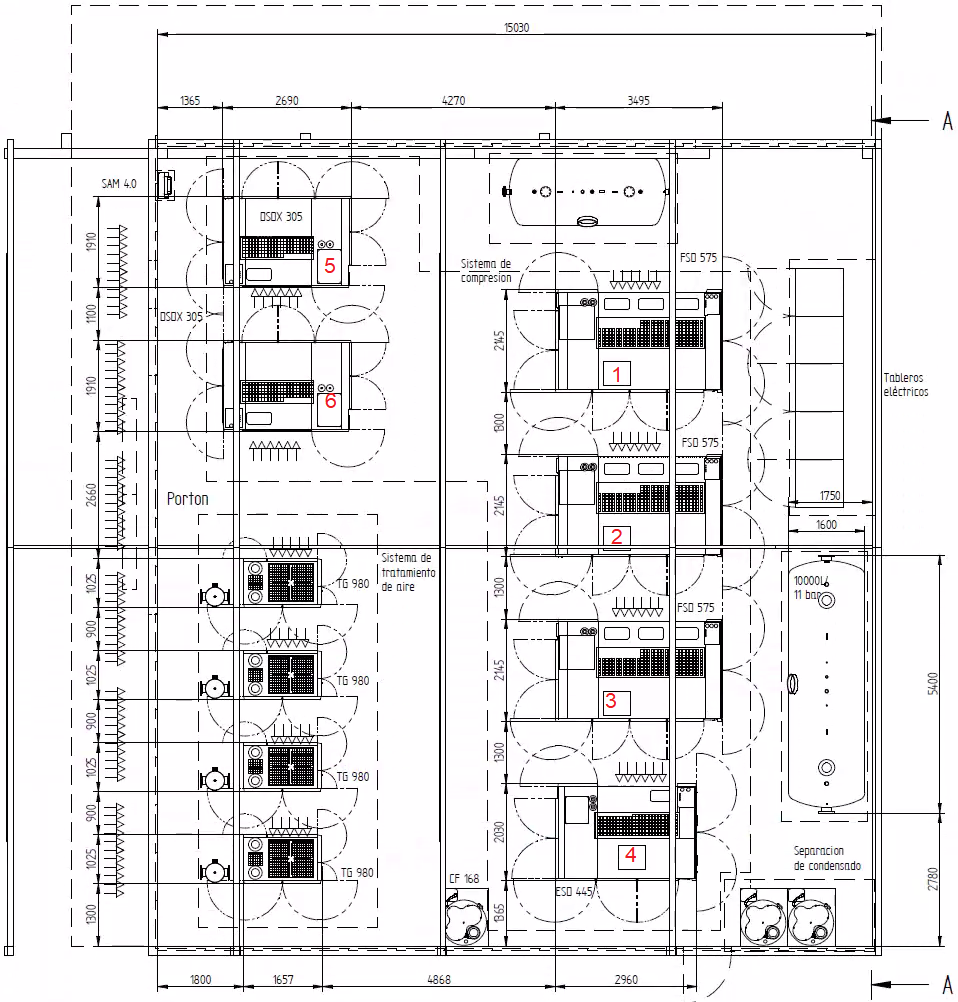
\includegraphics[width=0.8\linewidth]{img/plano_compresores.png}
    \caption{Plano de distribución de los compresores en la sala de máquinas.}
    \label{fig:layout_compresores}
\end{figure}

Estos anexos proporcionan una visión más completa y detallada de la información técnica y respaldan el informe de diseño del sistema de recuperación de calor para la planta de Papeles Cordillera S.A.
\newpage


\end{document}
